% Standalone source of the figure fig:ls9 of the Legendre-cell paper: the structure of the nine-component
% Lippmann--Schwinger equation, psi = psi0 + int Gcal(x - y) Delta psi(y) dy, drawn as block shapes.
% Build: pdflatex fig_ls9.tex; the paper includes the PDF. Grey scale only.
% One unit is one component. The state psi = (u, eps) has 3 + 6 components; the kernel's four blocks carry
% zero, one, one and two derivatives of the Green's tensor (shaded by their singularity); the contrast is
% block diagonal and turns the state into the sources: a force from the displacement, a moment from the strain.
\documentclass[border=2pt]{standalone}
% Shared preamble of the standalone figures of the Legendre-cell paper.
\usepackage{amsmath,amssymb,bm}
\usepackage{tikz}
\usetikzlibrary{calc,arrows.meta,decorations.pathreplacing}

\begin{document}
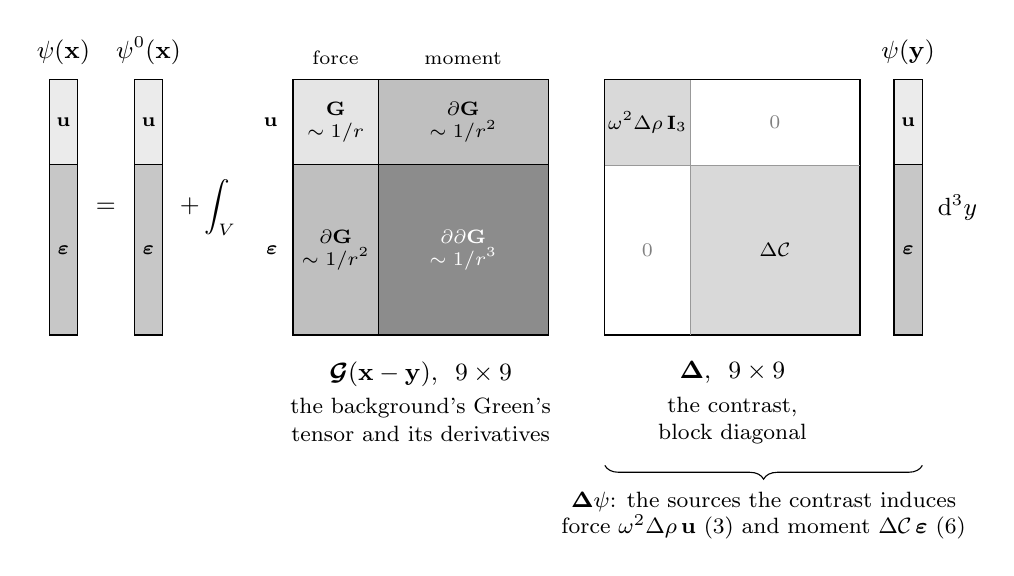
\begin{tikzpicture}[x=0.36cm, y=-0.36cm, >=Stealth, font=\small]
  % a state column (u above eps) with its left edge at x = #1
  \newcommand{\statecol}[2]{%
    \fill[black!8] (#1,0) rectangle (#1+1,3);
    \fill[black!22] (#1,3) rectangle (#1+1,9);
    \draw (#1,0) rectangle (#1+1,9);
    \draw (#1,3) -- (#1+1,3);
    \node[font=\scriptsize] at (#1+0.5,1.5) {$\mathbf u$};
    \node[font=\scriptsize] at (#1+0.5,6) {$\boldsymbol\varepsilon$};
    \node[anchor=south] at (#1+0.5,-0.2) {#2};
  }
  % ------------------------------------------------------------------ psi = psi0 +
  \statecol{0}{$\psi(\mathbf x)$}
  \node at (2,4.5) {$=$};
  \statecol{3}{$\psi^0(\mathbf x)$}
  \node at (5.6,4.5) {$+\displaystyle\int_V$};
  % ------------------------------------------------------------------ the kernel, 9 x 9
  \begin{scope}[shift={(8.6,0)}]
    \fill[black!10] (0,0) rectangle (3,3);
    \fill[black!25] (3,0) rectangle (9,3);
    \fill[black!25] (0,3) rectangle (3,9);
    \fill[black!45] (3,3) rectangle (9,9);
    \draw (0,0) rectangle (9,9);
    \draw (3,0) -- (3,9);
    \draw (0,3) -- (9,3);
    \node[align=center, font=\scriptsize] at (1.5,1.5) {$\mathbf G$\\$\sim1/r$};
    \node[align=center, font=\scriptsize] at (6,1.5) {$\partial\mathbf G$\\$\sim1/r^2$};
    \node[align=center, font=\scriptsize] at (1.5,6) {$\partial\mathbf G$\\$\sim1/r^2$};
    \node[align=center, font=\scriptsize, text=white] at (6,6) {$\partial\partial\mathbf G$\\$\sim1/r^3$};
    \node[font=\scriptsize, anchor=south] at (1.5,-0.2) {force};
    \node[font=\scriptsize, anchor=south] at (6,-0.2) {moment};
    \node[font=\scriptsize, anchor=east] at (-0.2,1.5) {$\mathbf u$};
    \node[font=\scriptsize, anchor=east] at (-0.2,6) {$\boldsymbol\varepsilon$};
    \node[anchor=north, align=center] at (4.5,9.6)
      {$\boldsymbol{\mathcal G}(\mathbf x-\mathbf y)$, \ $9\times9$\\[1pt]
       \footnotesize the background's Green's\\[-1pt]\footnotesize tensor and its derivatives};
  \end{scope}
  % ------------------------------------------------------------------ the contrast, 9 x 9 block diagonal
  \begin{scope}[shift={(19.6,0)}]
    \fill[black!15] (0,0) rectangle (3,3);
    \fill[black!15] (3,3) rectangle (9,9);
    \draw (0,0) rectangle (9,9);
    \draw[black!40, very thin] (3,0) -- (3,9);
    \draw[black!40, very thin] (0,3) -- (9,3);
    \node[font=\scriptsize] at (1.5,1.5) {$\omega^2\Delta\rho\,\mathbf I_3$};
    \node[font=\scriptsize] at (6,6) {$\Delta\mathcal C$};
    \node[font=\scriptsize, black!50] at (6,1.5) {$0$};
    \node[font=\scriptsize, black!50] at (1.5,6) {$0$};
    \node[anchor=north, align=center] at (4.5,9.6)
      {$\boldsymbol\Delta$, \ $9\times9$\\[1pt]\footnotesize the contrast,\\[-1pt]\footnotesize block diagonal};
  \end{scope}
  % ------------------------------------------------------------------ psi(y)
  \statecol{29.8}{$\psi(\mathbf y)$}
  \node[anchor=west] at (31,4.5) {$\mathrm d^3y$};
  % ------------------------------------------------------------------ what Delta psi is
  \draw[decorate, decoration={brace, amplitude=5pt, mirror}] (19.6,13.6) -- (30.8,13.6)
    node[midway, below=6pt, align=center, font=\footnotesize]
    {$\boldsymbol\Delta\psi$: the sources the contrast induces\\
     force $\omega^2\Delta\rho\,\mathbf u$ (3) and moment $\Delta\mathcal C\,\boldsymbol\varepsilon$ (6)};
\end{tikzpicture}
\end{document}
